\documentclass[compress]{beamer}
\usepackage{ifthen,verbatim}

\title{Simulation of disk/wheel alignment \\ with systematics studies}
\author{Jim Pivarski, Alexei Safonov}
\institute{Texas A\&M University}
\date{ 6 August, 2007}

\newcommand{\isnote}{}
\xdefinecolor{lightyellow}{rgb}{1.,1.,0.25}
\xdefinecolor{darkblue}{rgb}{0.1,0.1,0.7}

%% Uncomment this to get annotations
%% \def\notes{\addtocounter{page}{-1}
%%            \renewcommand{\isnote}{*}
%% 	   \beamertemplateshadingbackground{lightyellow}{white}
%%            \begin{frame}
%%            \frametitle{Notes for the previous page (page \insertpagenumber)}
%%            \itemize}
%% \def\endnotes{\enditemize
%% 	      \end{frame}
%%               \beamertemplateshadingbackground{white}{white}
%%               \renewcommand{\isnote}{}}

%% Uncomment this to not get annotations
\def\notes{\comment}
\def\endnotes{\endcomment}

\setbeamertemplate{navigation symbols}{}
\setbeamertemplate{headline}{\includegraphics[height=1 cm]{../cmslogo} \hspace{0.1 cm} \includegraphics[height=1 cm]{../tamulogo} \hfill
\begin{minipage}{5.5 cm}
\vspace{-0.75 cm} \small
\begin{center}
\ifthenelse{\equal{\insertpagenumber}{1}}{}{\textcolor{blue}{\insertsection}}
\end{center}
\end{minipage} \hfill
\begin{minipage}{4.5 cm}
\vspace{-0.75 cm} \small
\begin{flushright}
\ifthenelse{\equal{\insertpagenumber}{1}}{}{Jim Pivarski \hspace{0.5 cm} \insertpagenumber\isnote/\pageref{numpages}}
\end{flushright}
\end{minipage}\mbox{\hspace{0.2 cm}}}

\begin{document}
\frame{\titlepage}

\begin{notes}
\item This is the annotated version of my talk.
\item If you want the version that I am presenting, download the one
labeled ``slides'' on Indico (or just ignore these yellow pages).
\item The annotated version is provided for extra detail and a written
record of comments that I intend to make orally.
\item Yellow notes refer to the content on the {\it previous} page.
\item All other slides are identical for the two versions.
\end{notes}

\begin{frame}
\frametitle{Advertisement: Available data in 1\_5\_2}
\begin{itemize}
\item 5000 $Z\to\mu\mu$

{\center \small /castor/cern.ch/user/p/pivarski/AlCaRecoMu/1\_5\_2/zmumu.root}

(this is what I used for the following study)

\vfill
\item 15$\times$ more single-mu

{\center \small /castor/cern.ch/user/p/pivarski/AlCaRecoMu/1\_5\_2/singlemu/*}
\end{itemize}
\end{frame}

\begin{frame}
\frametitle{Disk/Wheel alignment with internal misalignments}
\begin{itemize}\setlength{\itemsep}{0.25 cm}
  \item CSC Layers $\Delta x = 191$ $\mu$m, $\Delta y = 335$ $\mu$m, $\Delta \phi_z = 40$ $\mu$rad
  \item All Chambers $\Delta x = \Delta y = \Delta z = 3$ mm, \\ \mbox{ } \hfill $\Delta \phi_x = \Delta \phi_y = \Delta \phi_z = 1$ mrad
  \item Disks/wheels $\Delta x = \Delta y = \Delta z = 1$ cm, \\ \mbox{ } \hfill $\Delta \phi_x = \Delta \phi_y = \Delta \phi_z = 1$ mrad
  \item Tracker 10 pb$^{-1}$ scenario
\end{itemize}

\vfill
\begin{itemize}\setlength{\itemsep}{0.25 cm}
  \item Align muon system to tracker with globalMuons: $x$, $y$, $\phi_z$
\begin{itemize}
  \item Check dependence on tracker alignment
\end{itemize}

  \item Nominally 2000 $Z\to\mu\mu$ (0.36 pb$^{-1}$)
\begin{itemize}
  \item Check dependence on statistics
\end{itemize}
\end{itemize}
\end{frame}

\begin{frame}
\frametitle{Nominal case}
\begin{itemize}
\item Resolution is $\frac{1}{4}$ mrad due to internal misalignments

\item The end of this alignment is a starting point for chamber-by-chamber alignments
\end{itemize}
\begin{center}
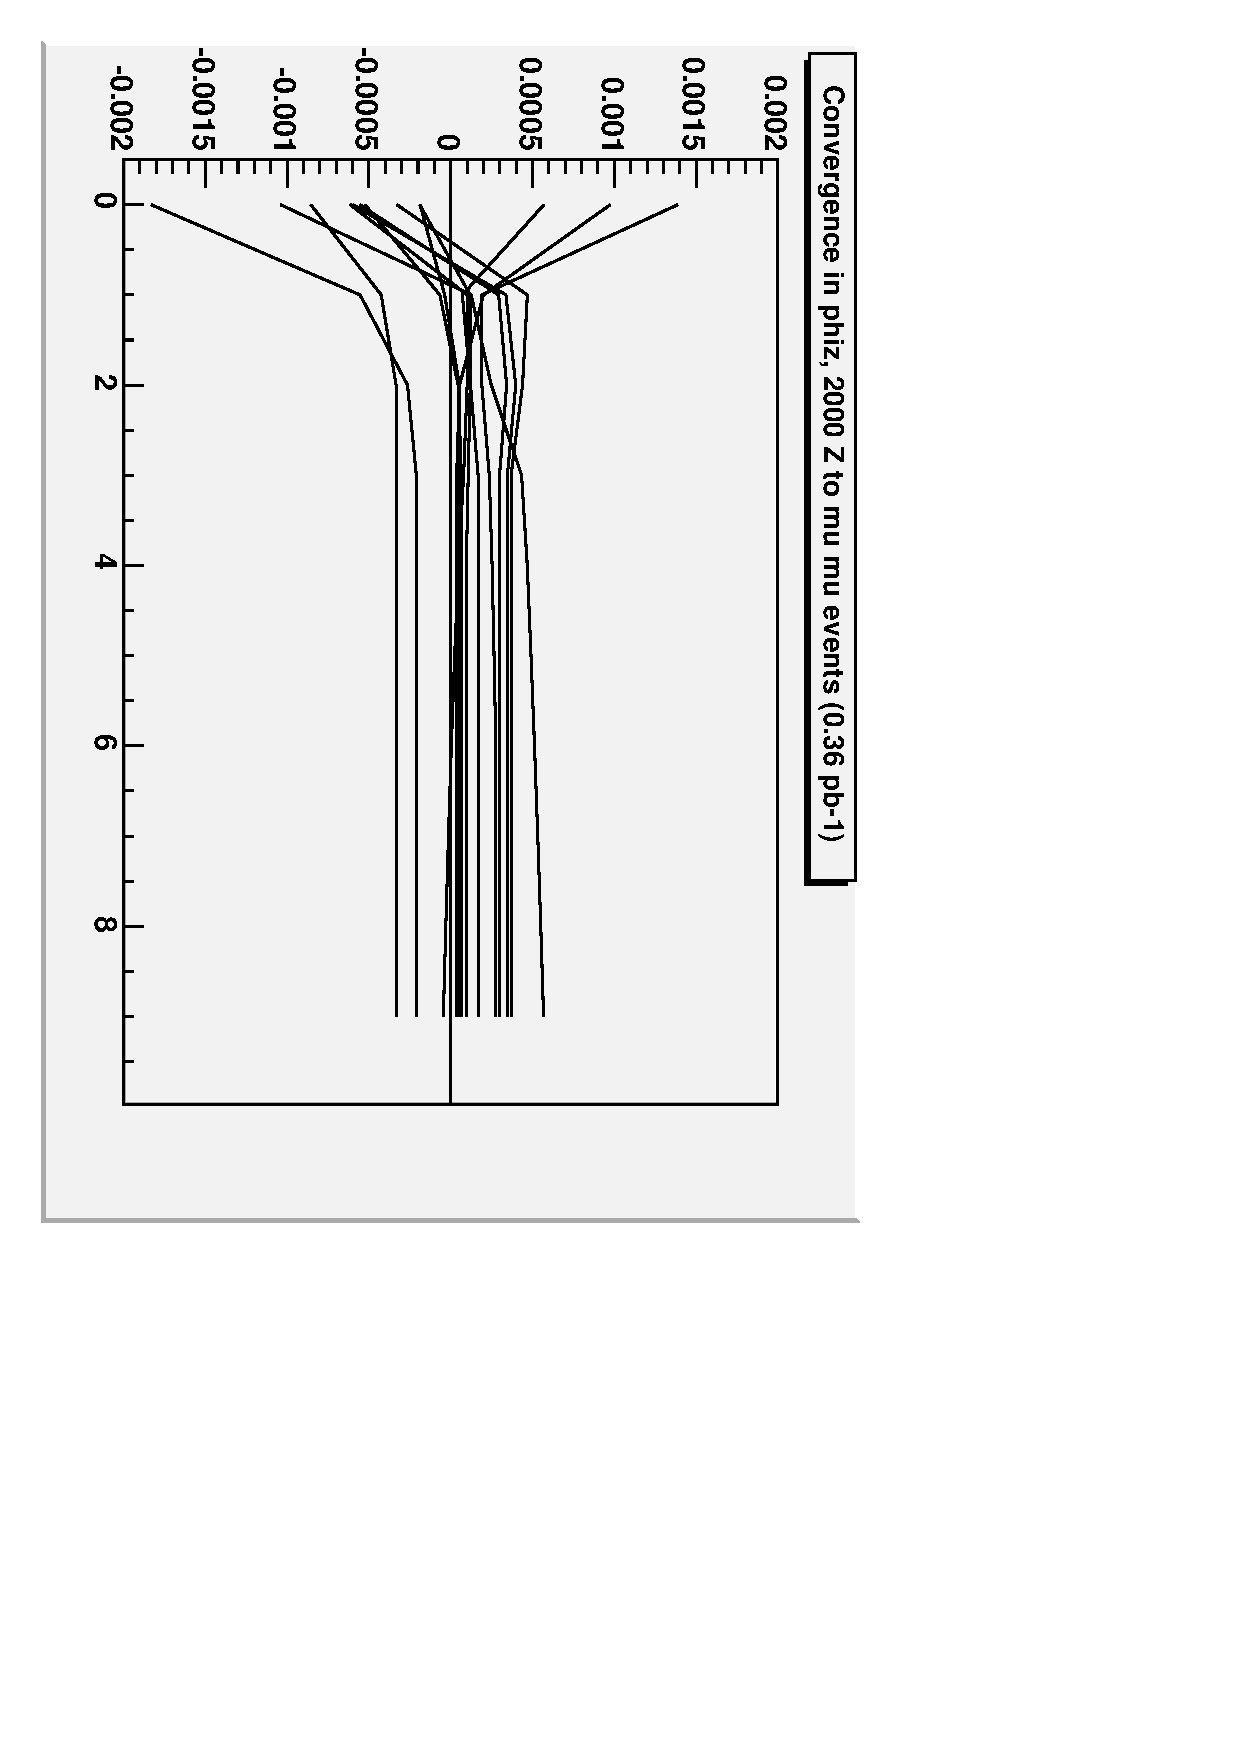
\includegraphics[height=0.7\linewidth, angle=90]{phiz_conv_2000.pdf}
\end{center}
\end{frame}

\begin{frame}
\frametitle{Is the simulation sensitive to tracker alignment? Yes!}
\begin{itemize}
\item Roll tracker 1 mrad with tracks tightly fit to it

\item Discovered that RPC hits will bias alignments toward ideal: we must always remove them!
\end{itemize}
\begin{center}
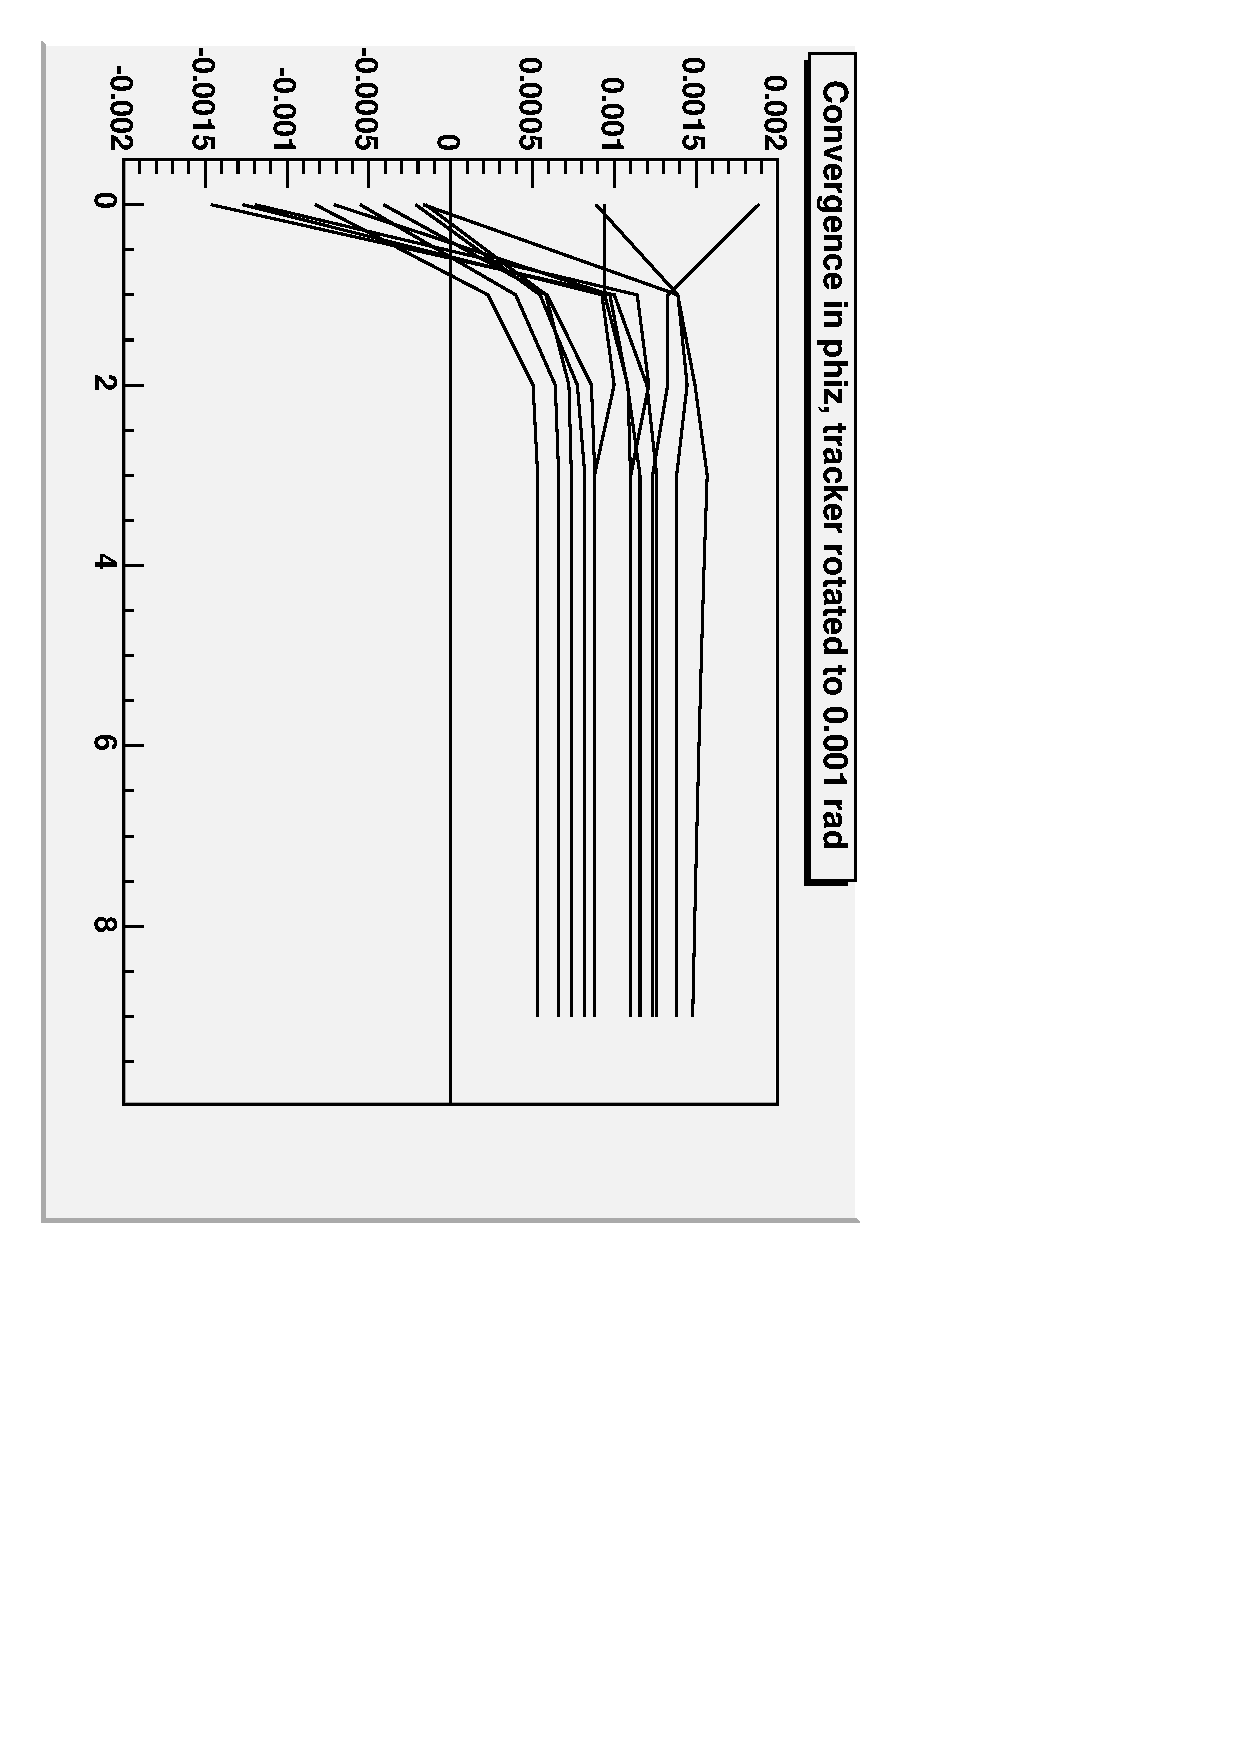
\includegraphics[height=0.7\linewidth, angle=90]{phiz_conv_barrel_roll.pdf}
\end{center}
\end{frame}

\begin{frame}
\frametitle{Multiply the tracker misalignment by 0, 2, 5, 10}
\begin{center}
\begin{tabular}{p{0.45\linewidth} p{0.45\linewidth}}
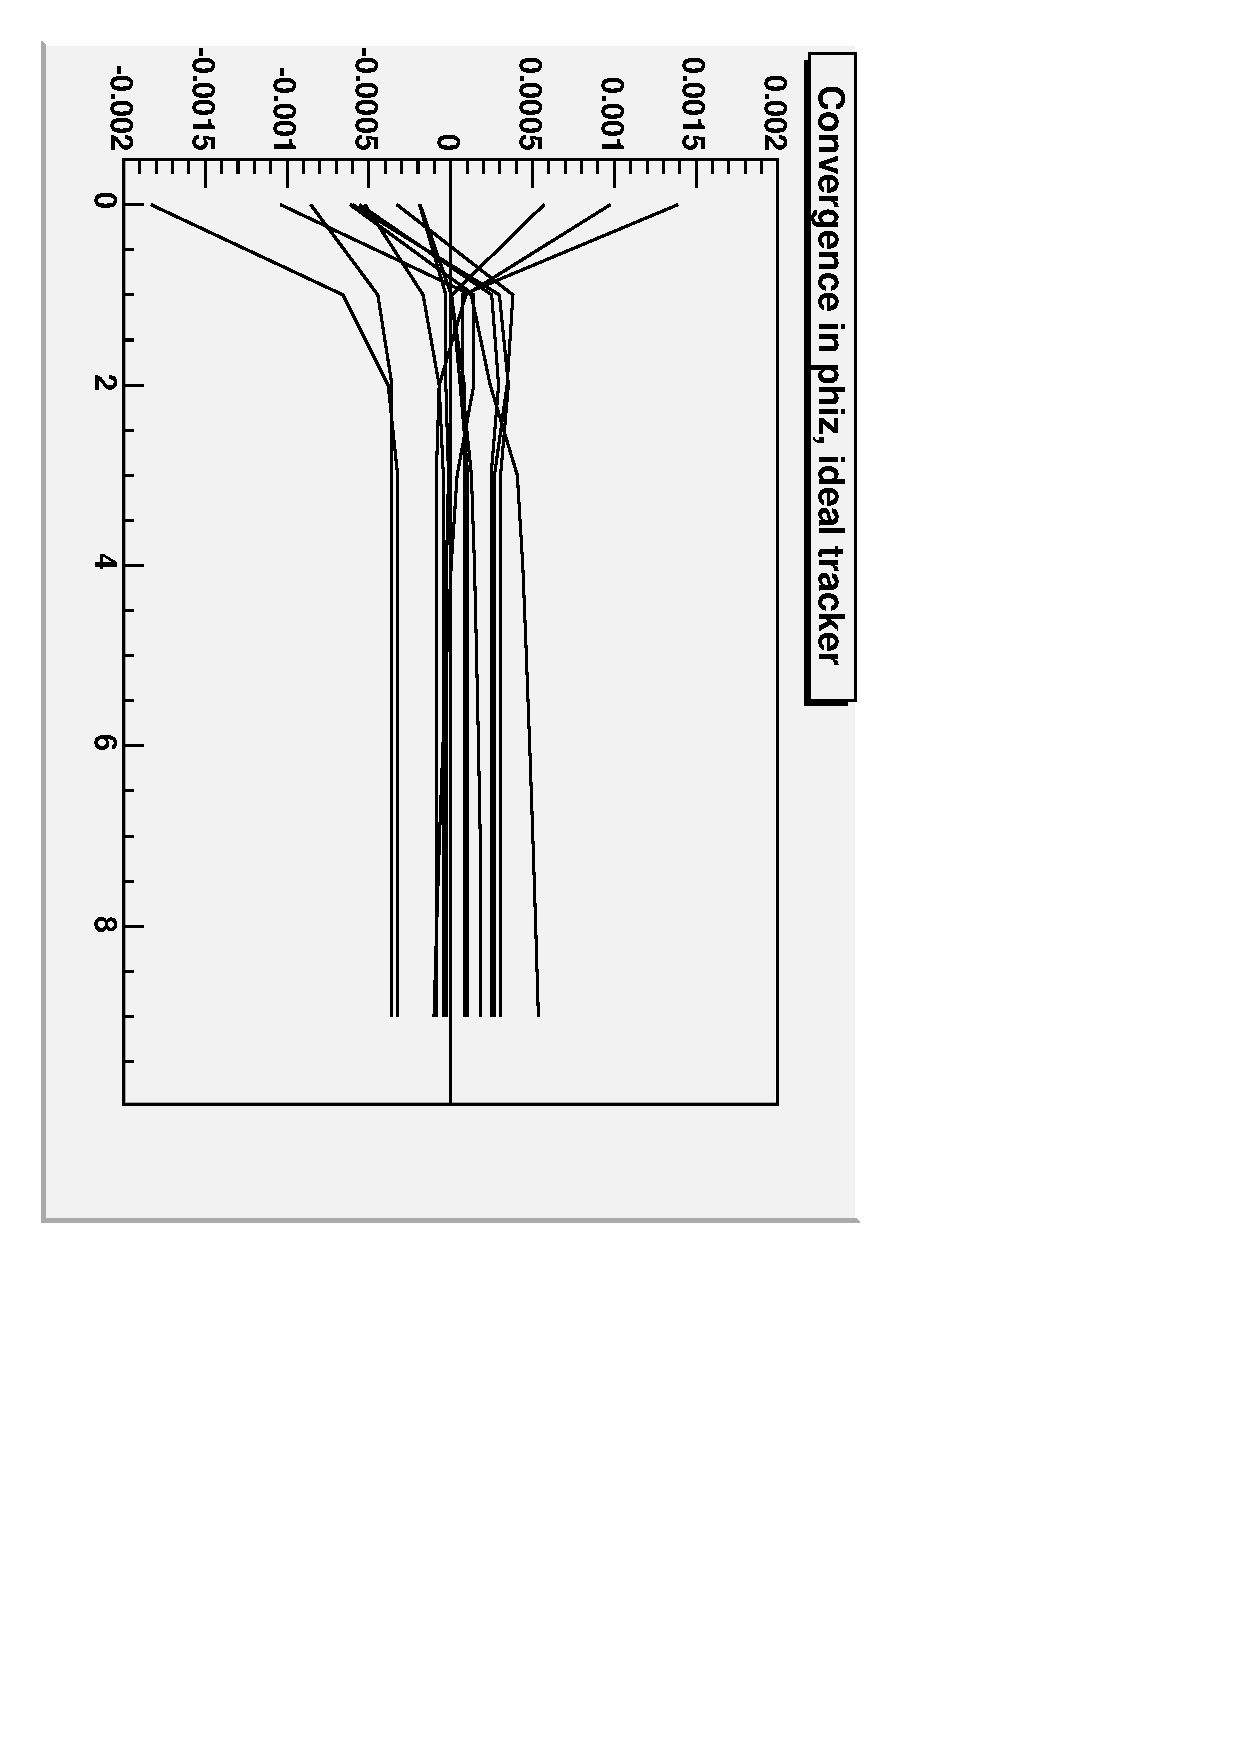
\includegraphics[height=\linewidth, angle=90]{phiz_conv_ideal_tracker.pdf} &
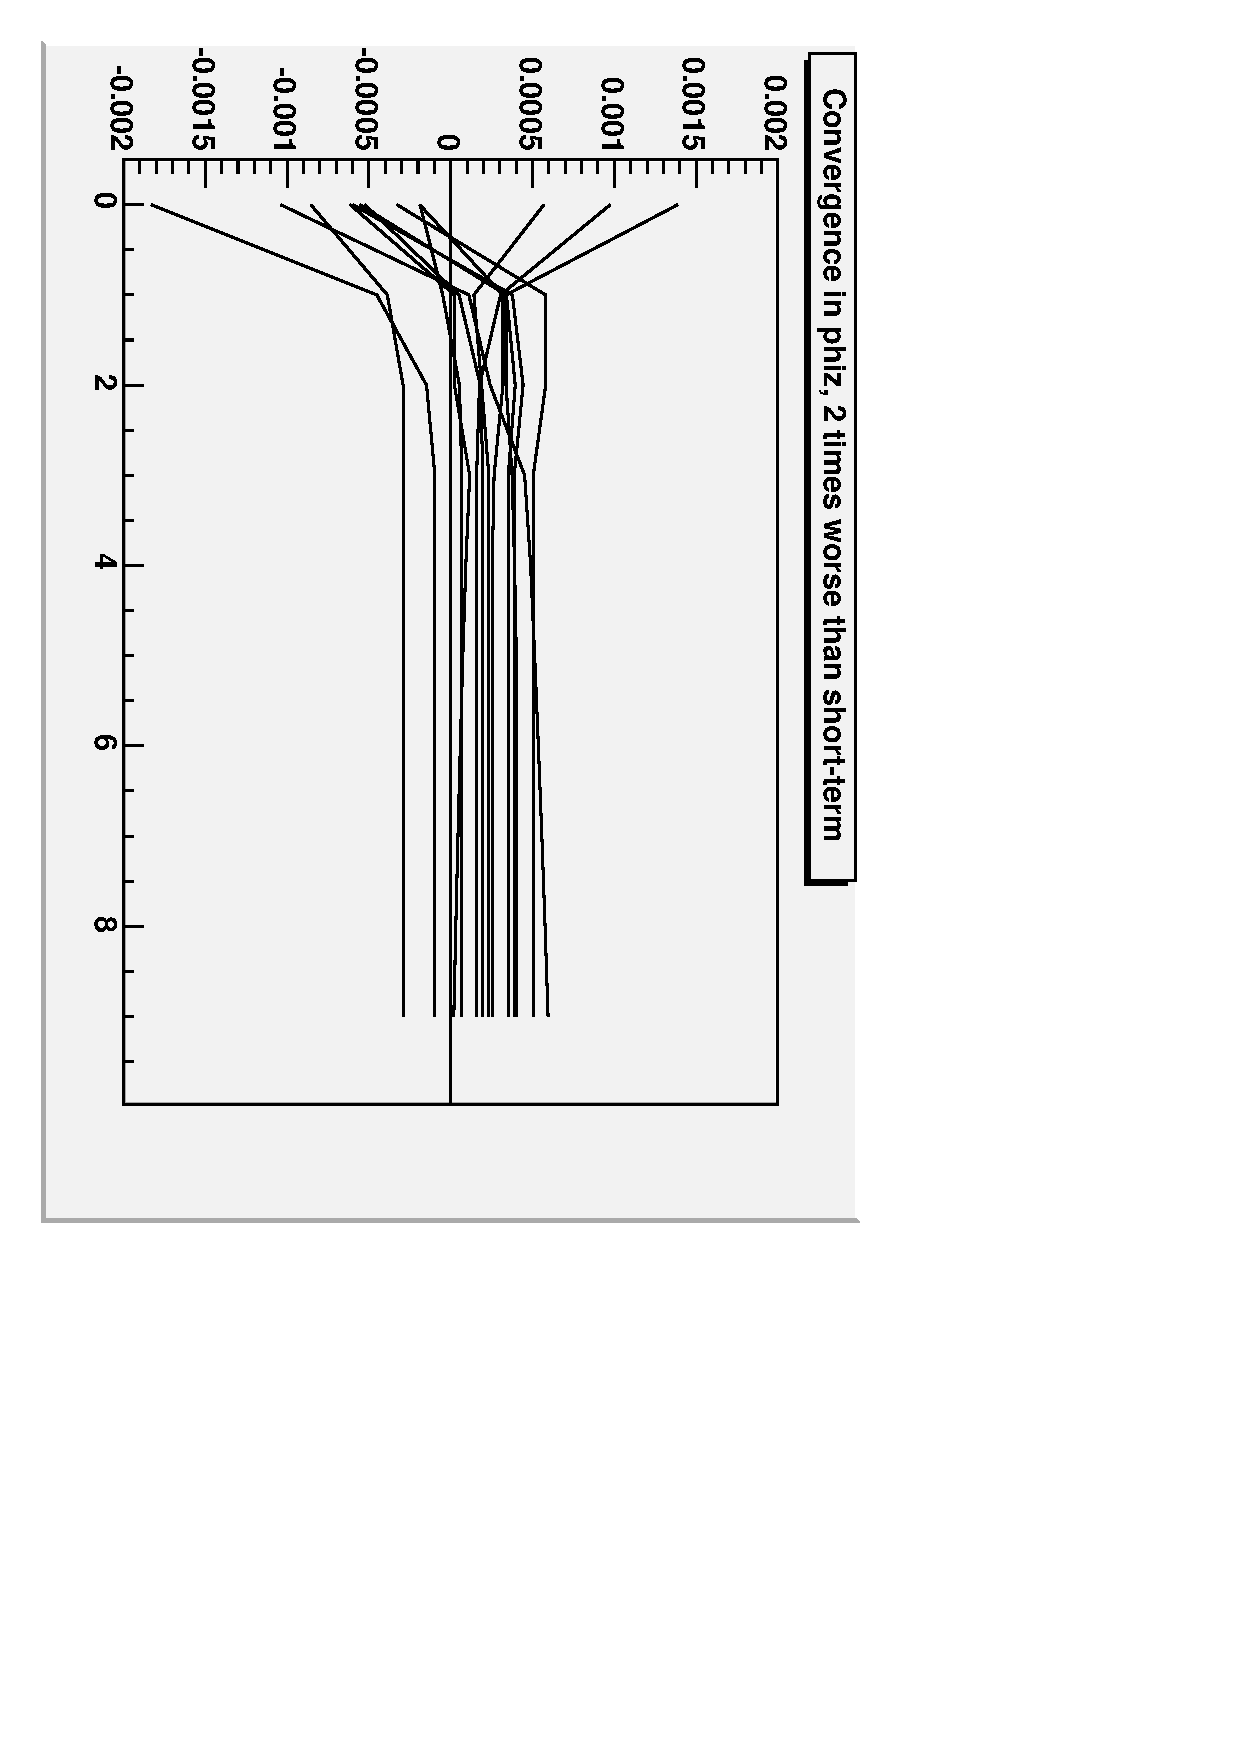
\includegraphics[height=\linewidth, angle=90]{phiz_conv_times2.pdf} \\
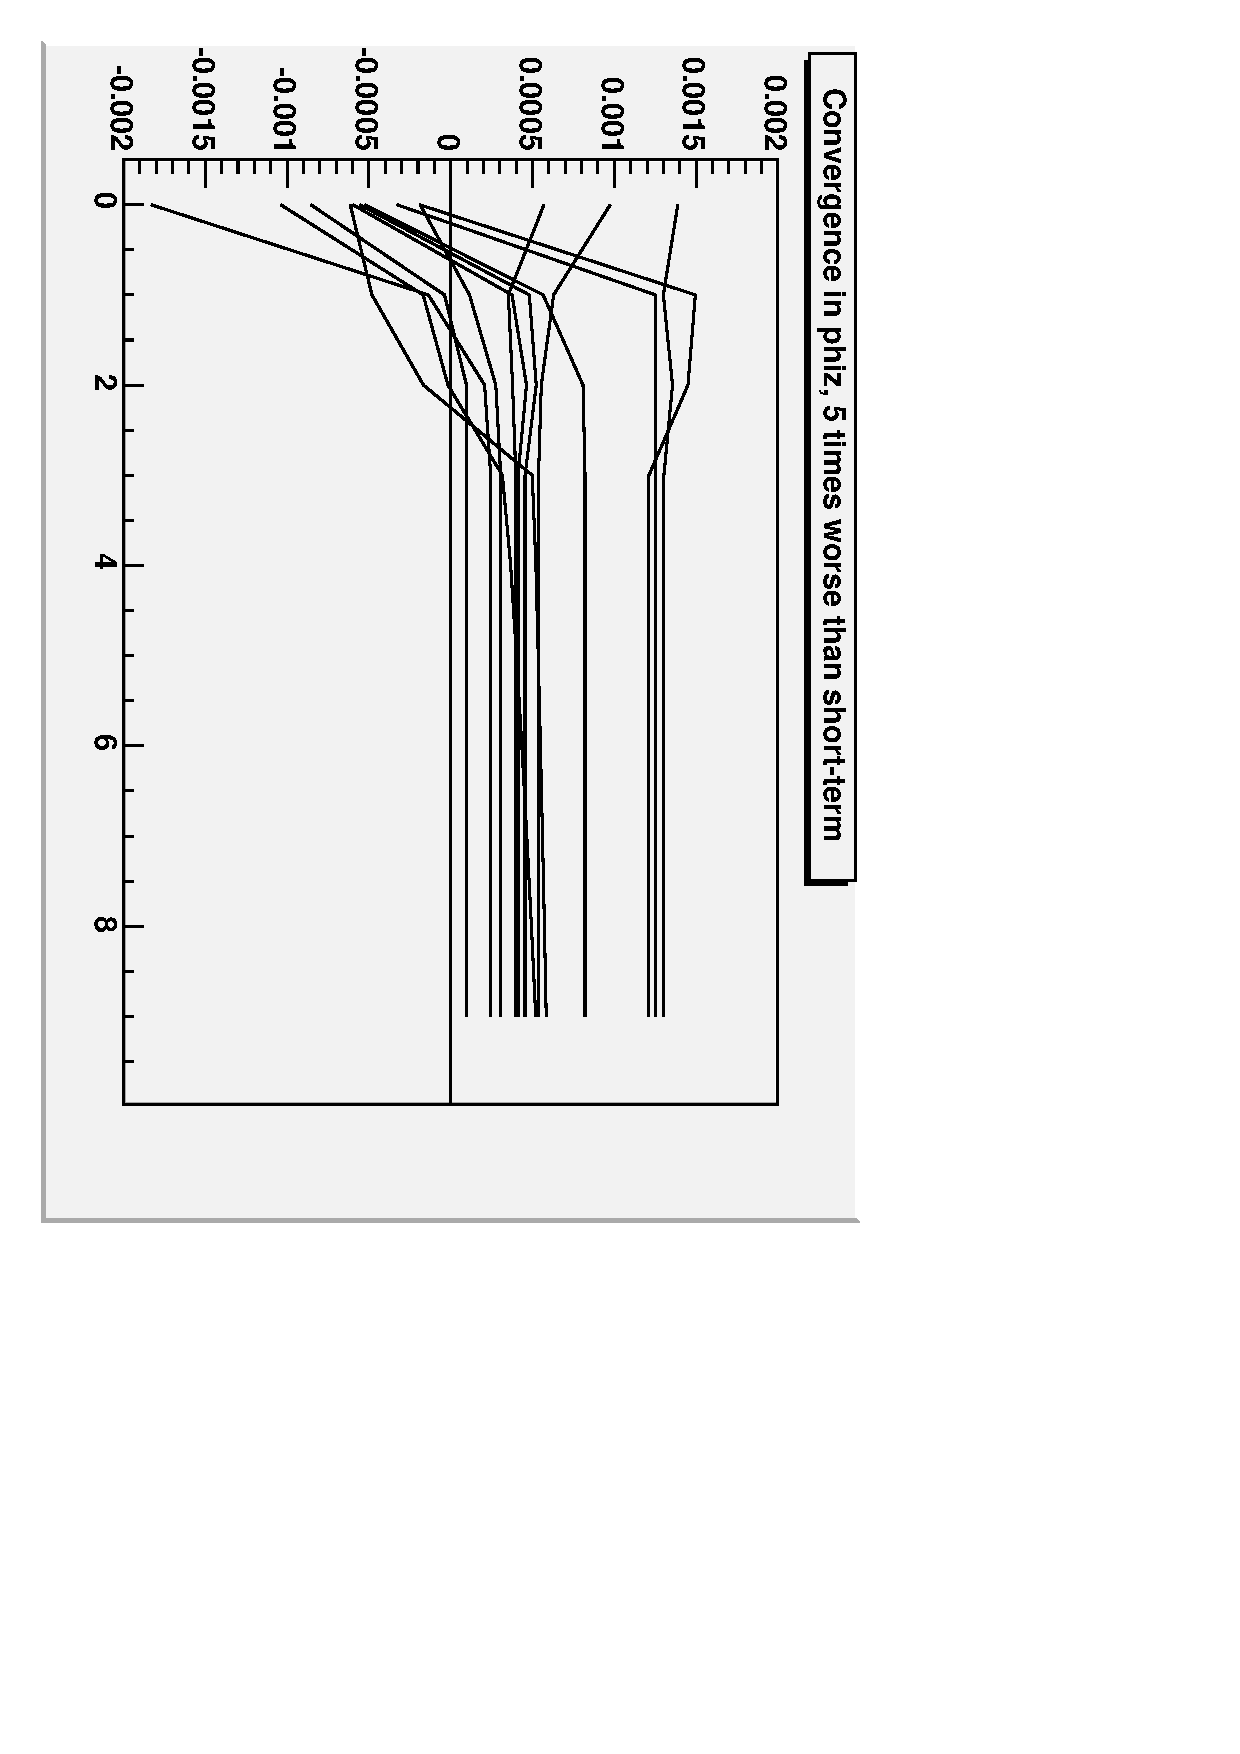
\includegraphics[height=\linewidth, angle=90]{phiz_conv_times5.pdf} &
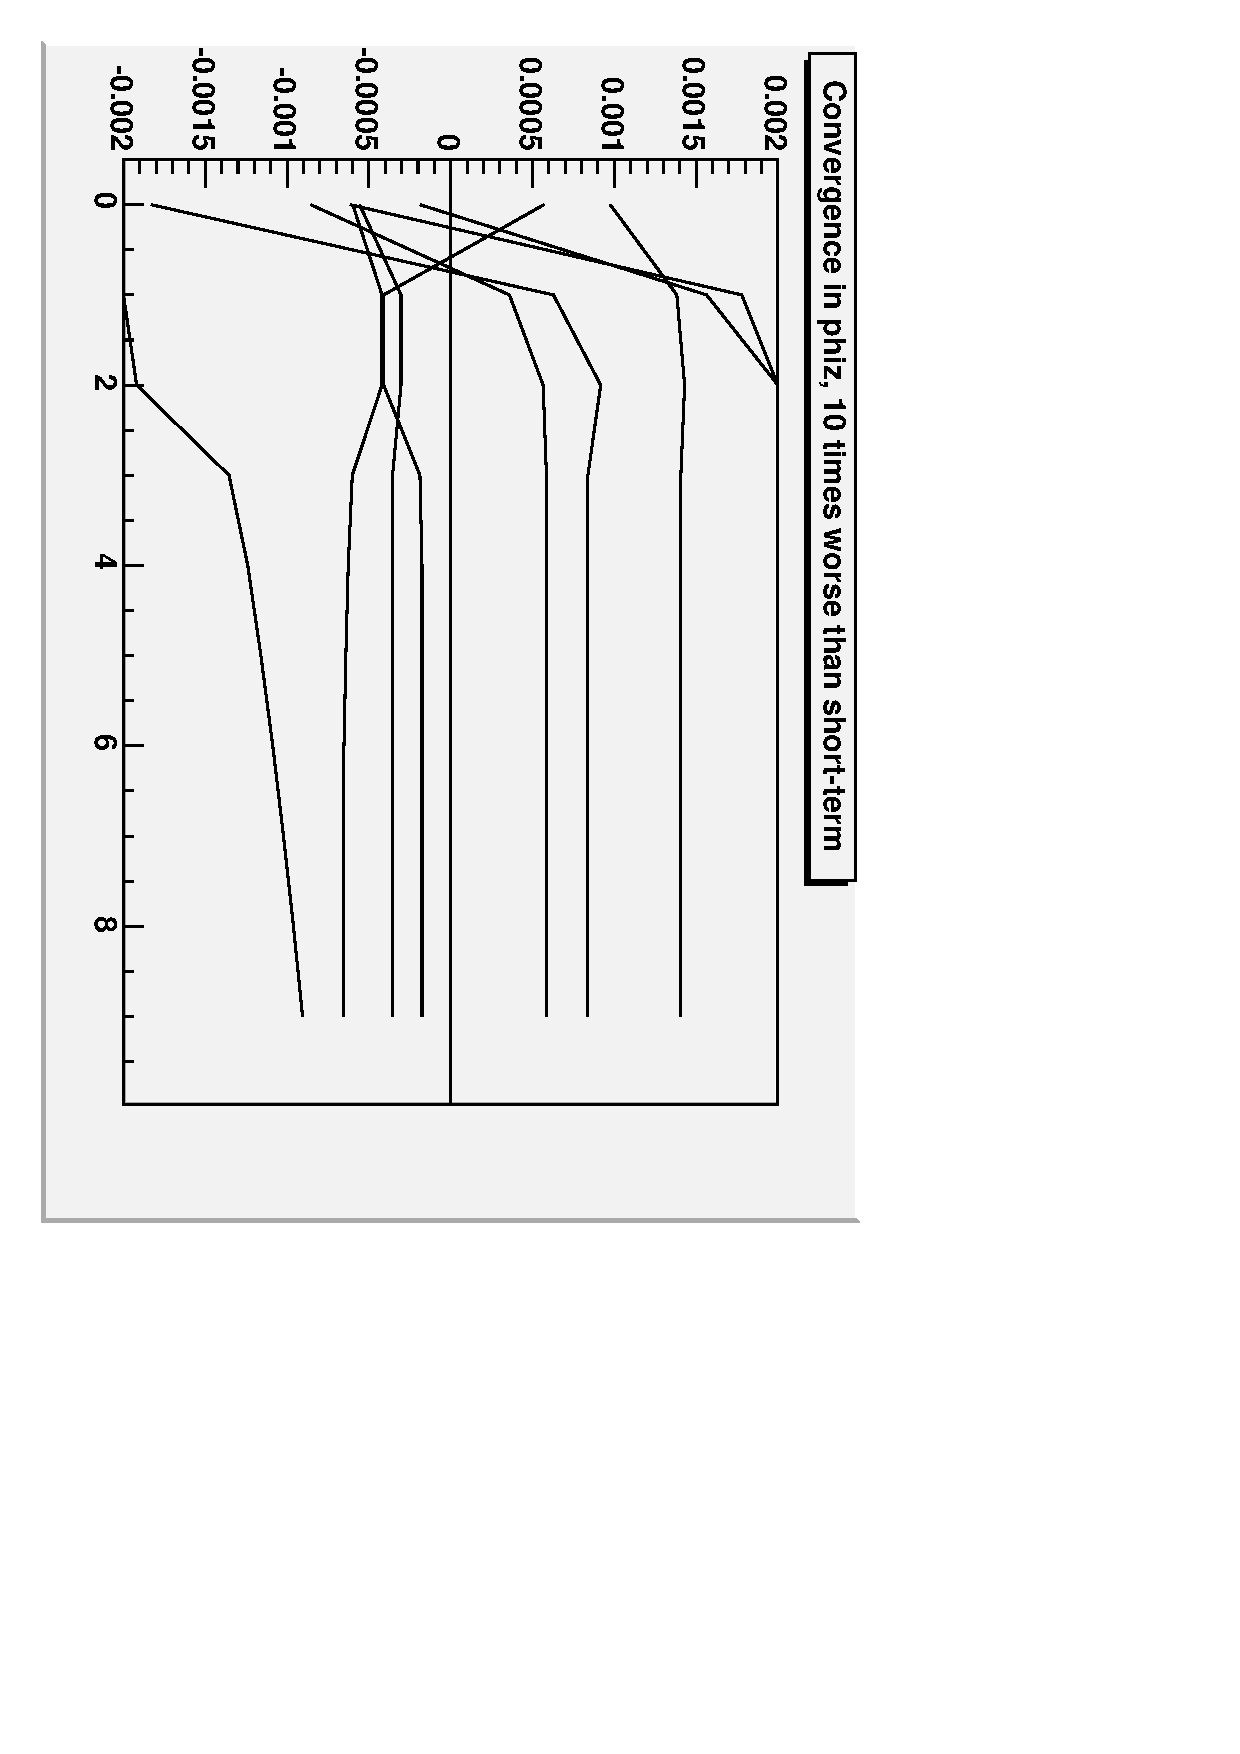
\includegraphics[height=\linewidth, angle=90]{phiz_conv_times10.pdf}
\end{tabular}
\end{center}
\end{frame}

\begin{frame}
\frametitle{Muon alignment quality vs tracker misalignment}
\begin{itemize}
\item RMS (not stdev!) of 13 disk/wheels times 10 trials, randomizing
muon alignment with each trial
\end{itemize}

\vfill
\begin{center}
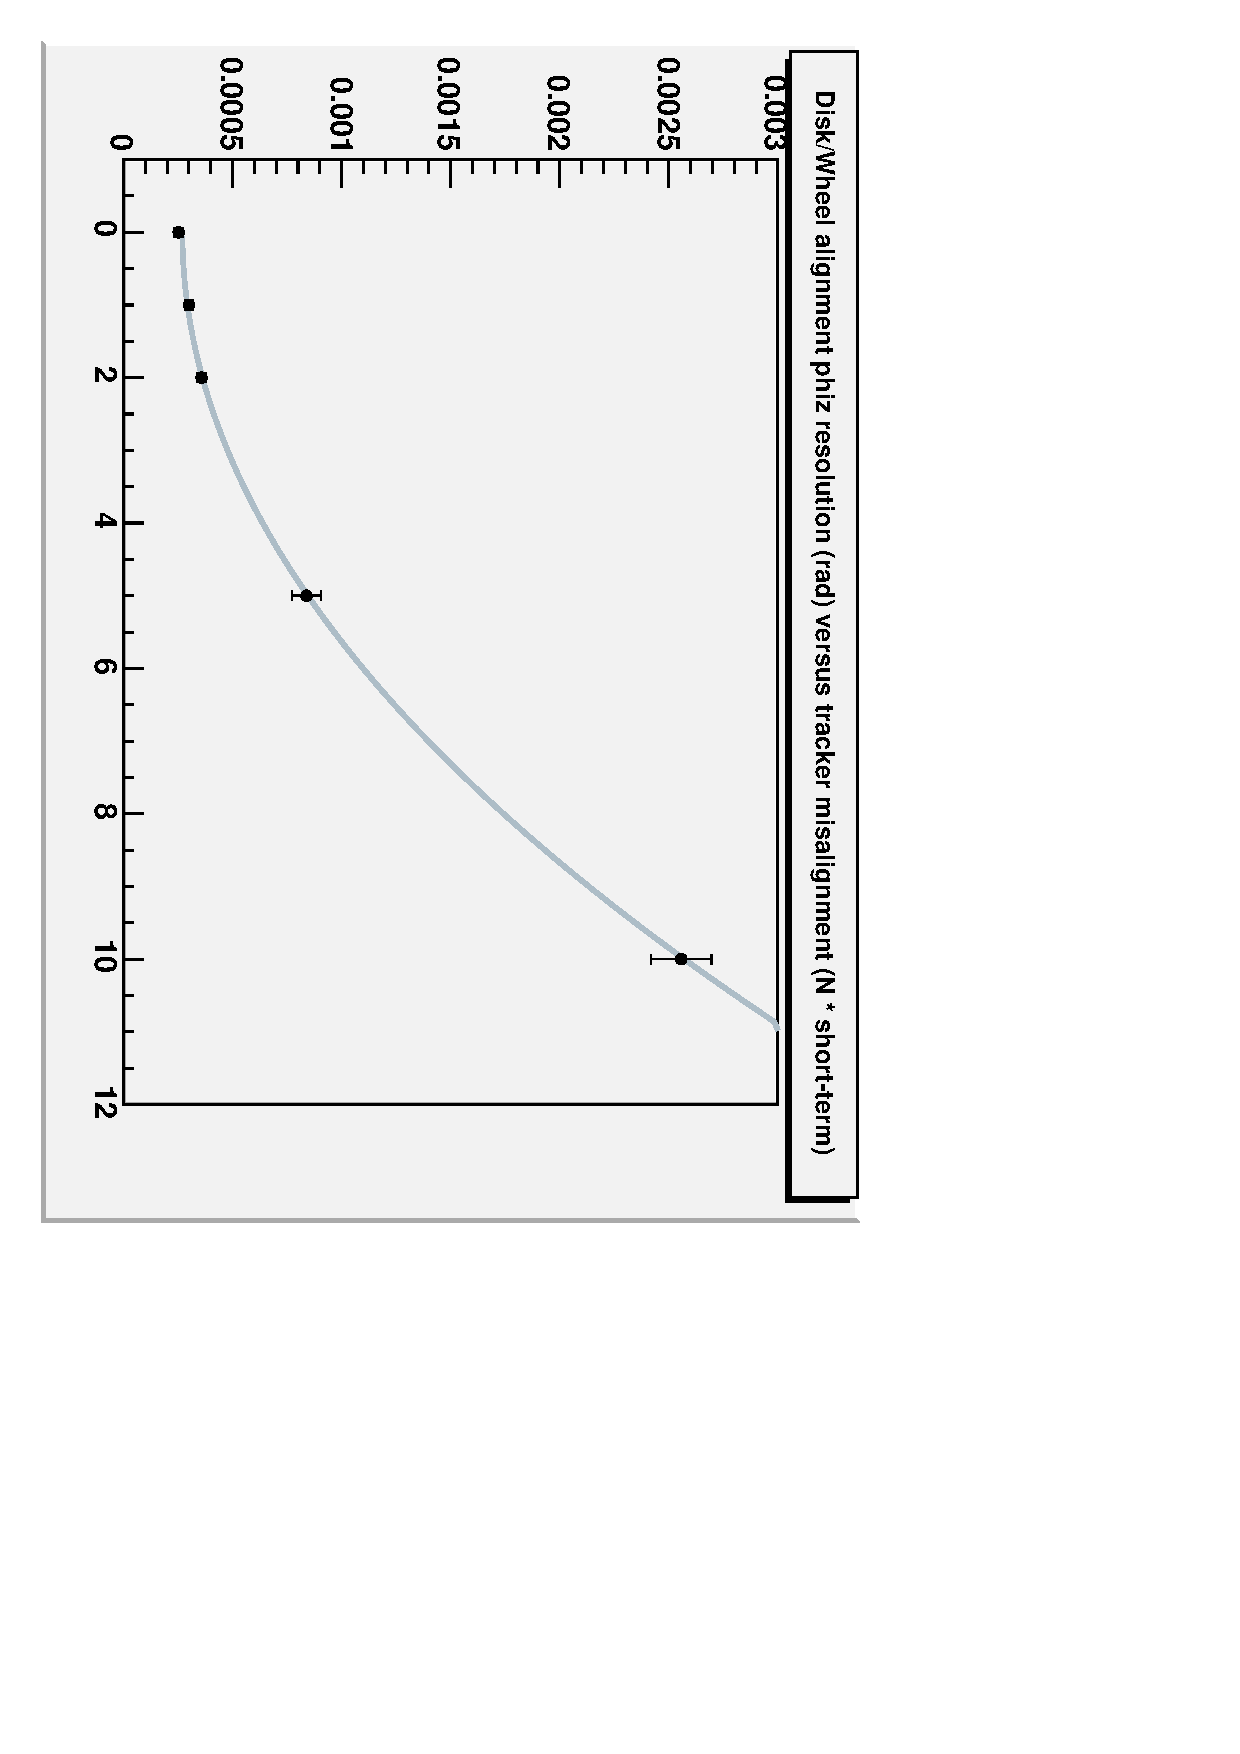
\includegraphics[height=0.6\linewidth, angle=90]{vstracker.pdf}
\end{center}

\vfill \center $\mbox{fit}(x) = 0.00027 + 0.000023 x^2$ ($\chi^2$ is too good because tracker trials are scaled up, not re-randomized)
\end{frame}

\begin{frame}
\frametitle{Reduce statistics: $1\times$, $\frac{1}{2}\times$, $\frac{1}{4}\times$, $\frac{1}{8}\times$}
\begin{center}
\begin{tabular}{p{0.45\linewidth} p{0.45\linewidth}}
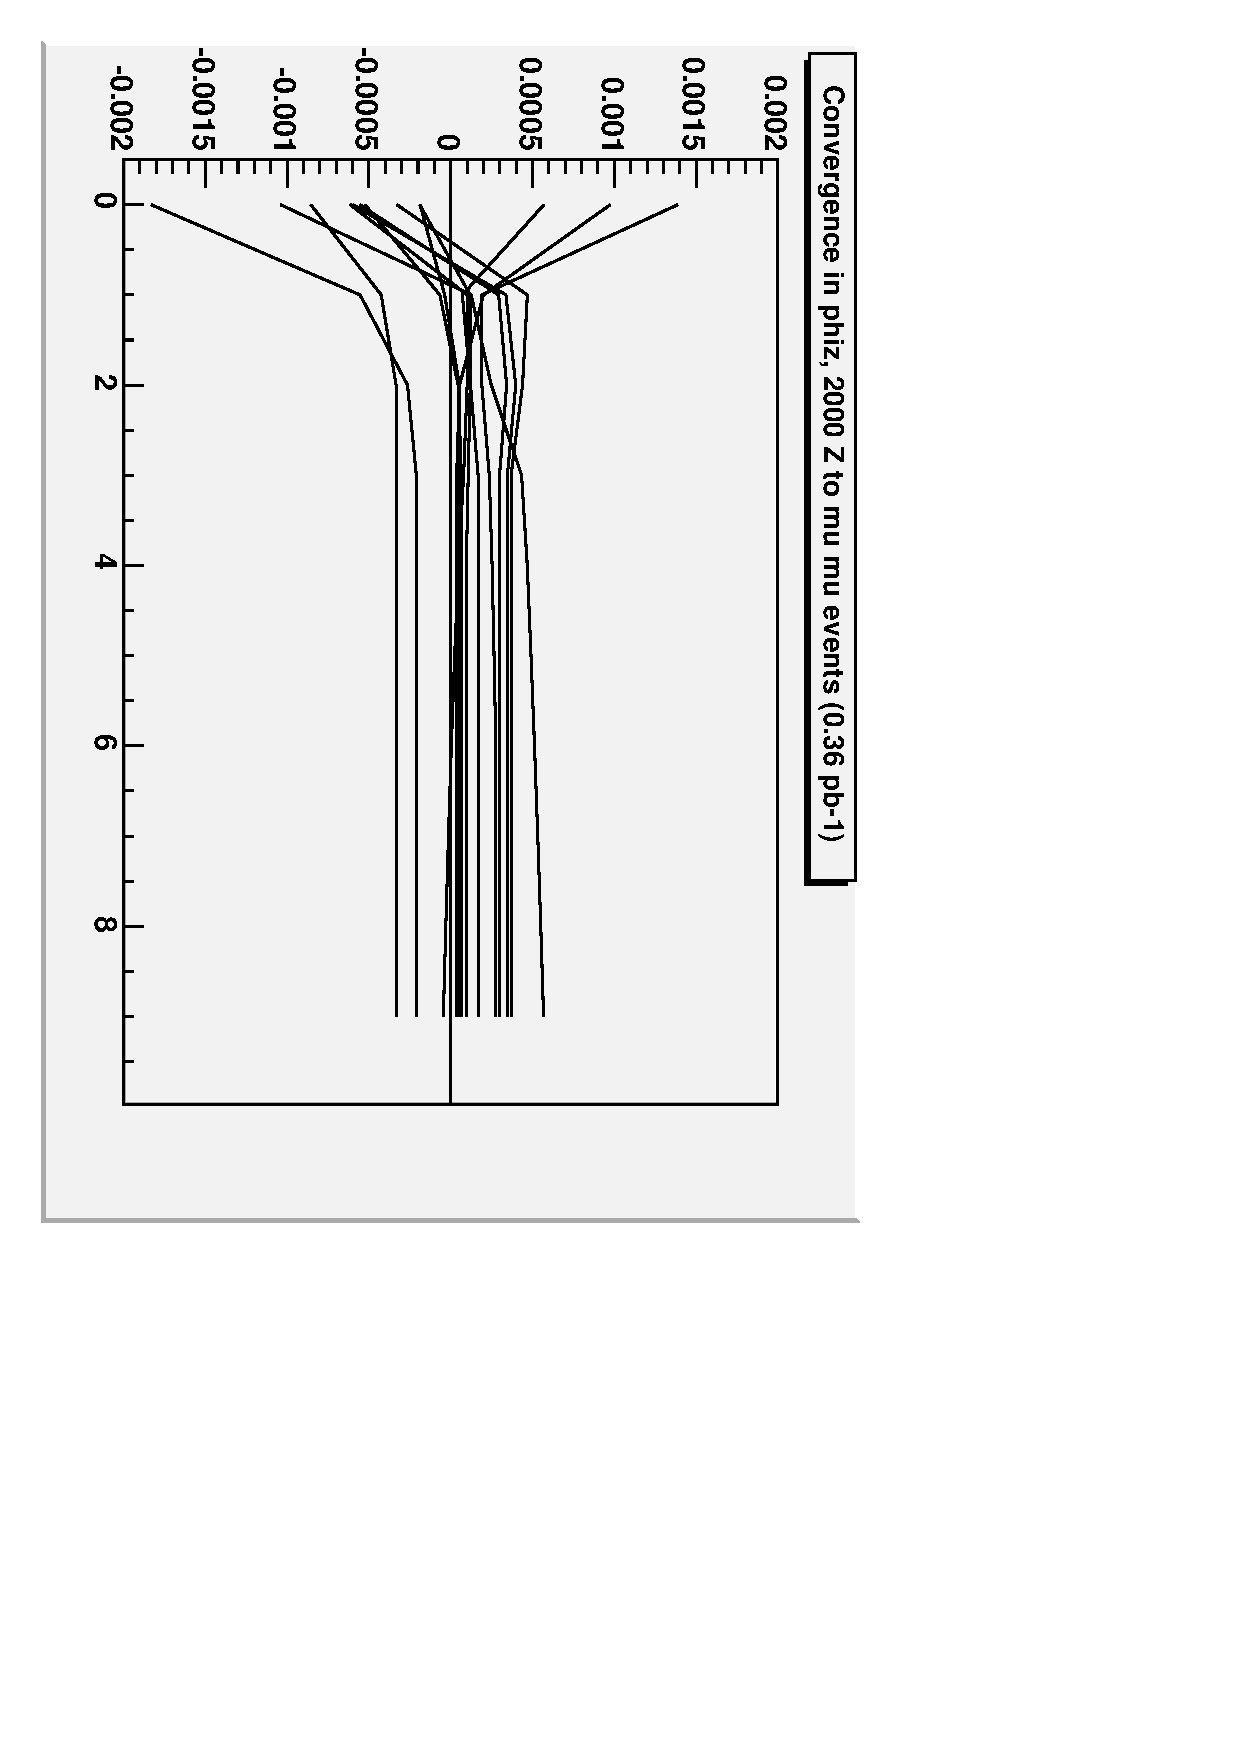
\includegraphics[height=\linewidth, angle=90]{phiz_conv_2000.pdf} &
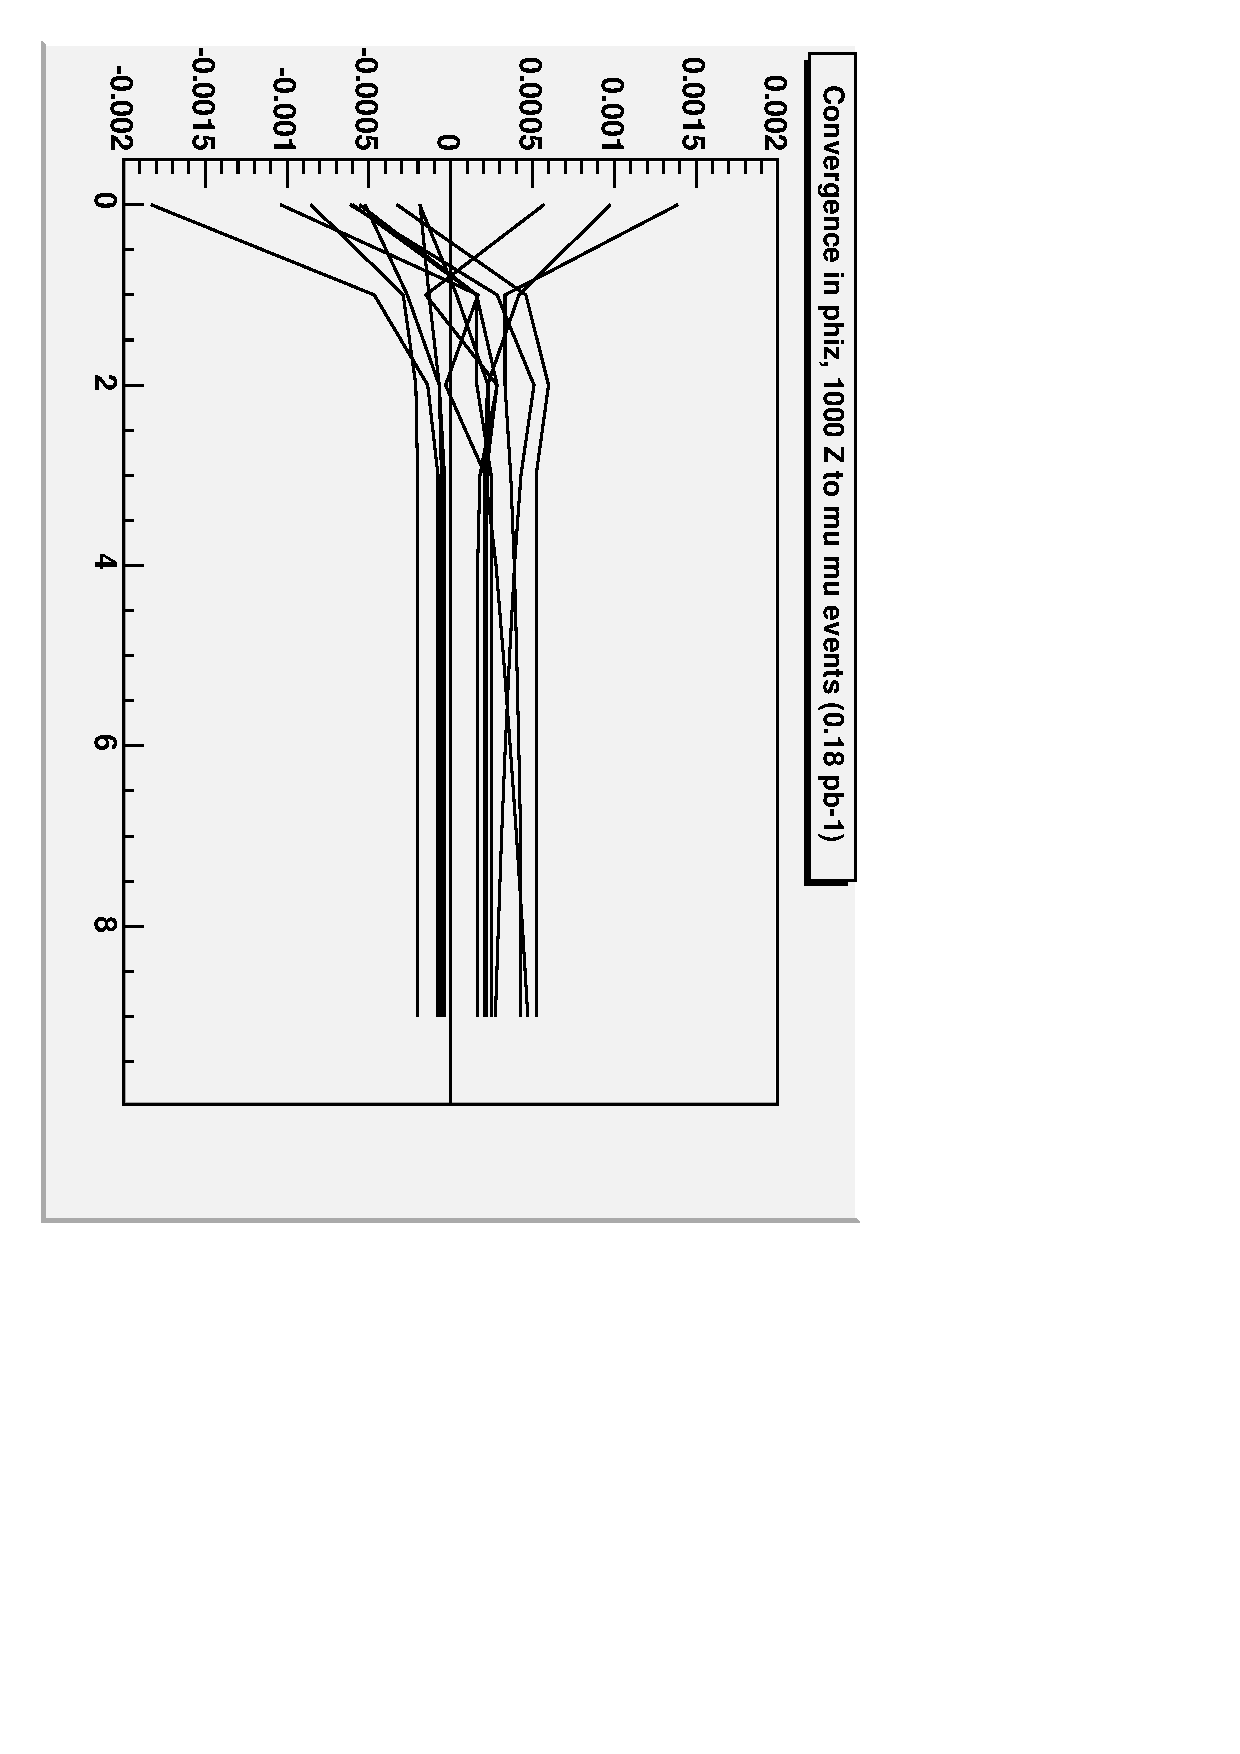
\includegraphics[height=\linewidth, angle=90]{phiz_conv_1000.pdf} \\
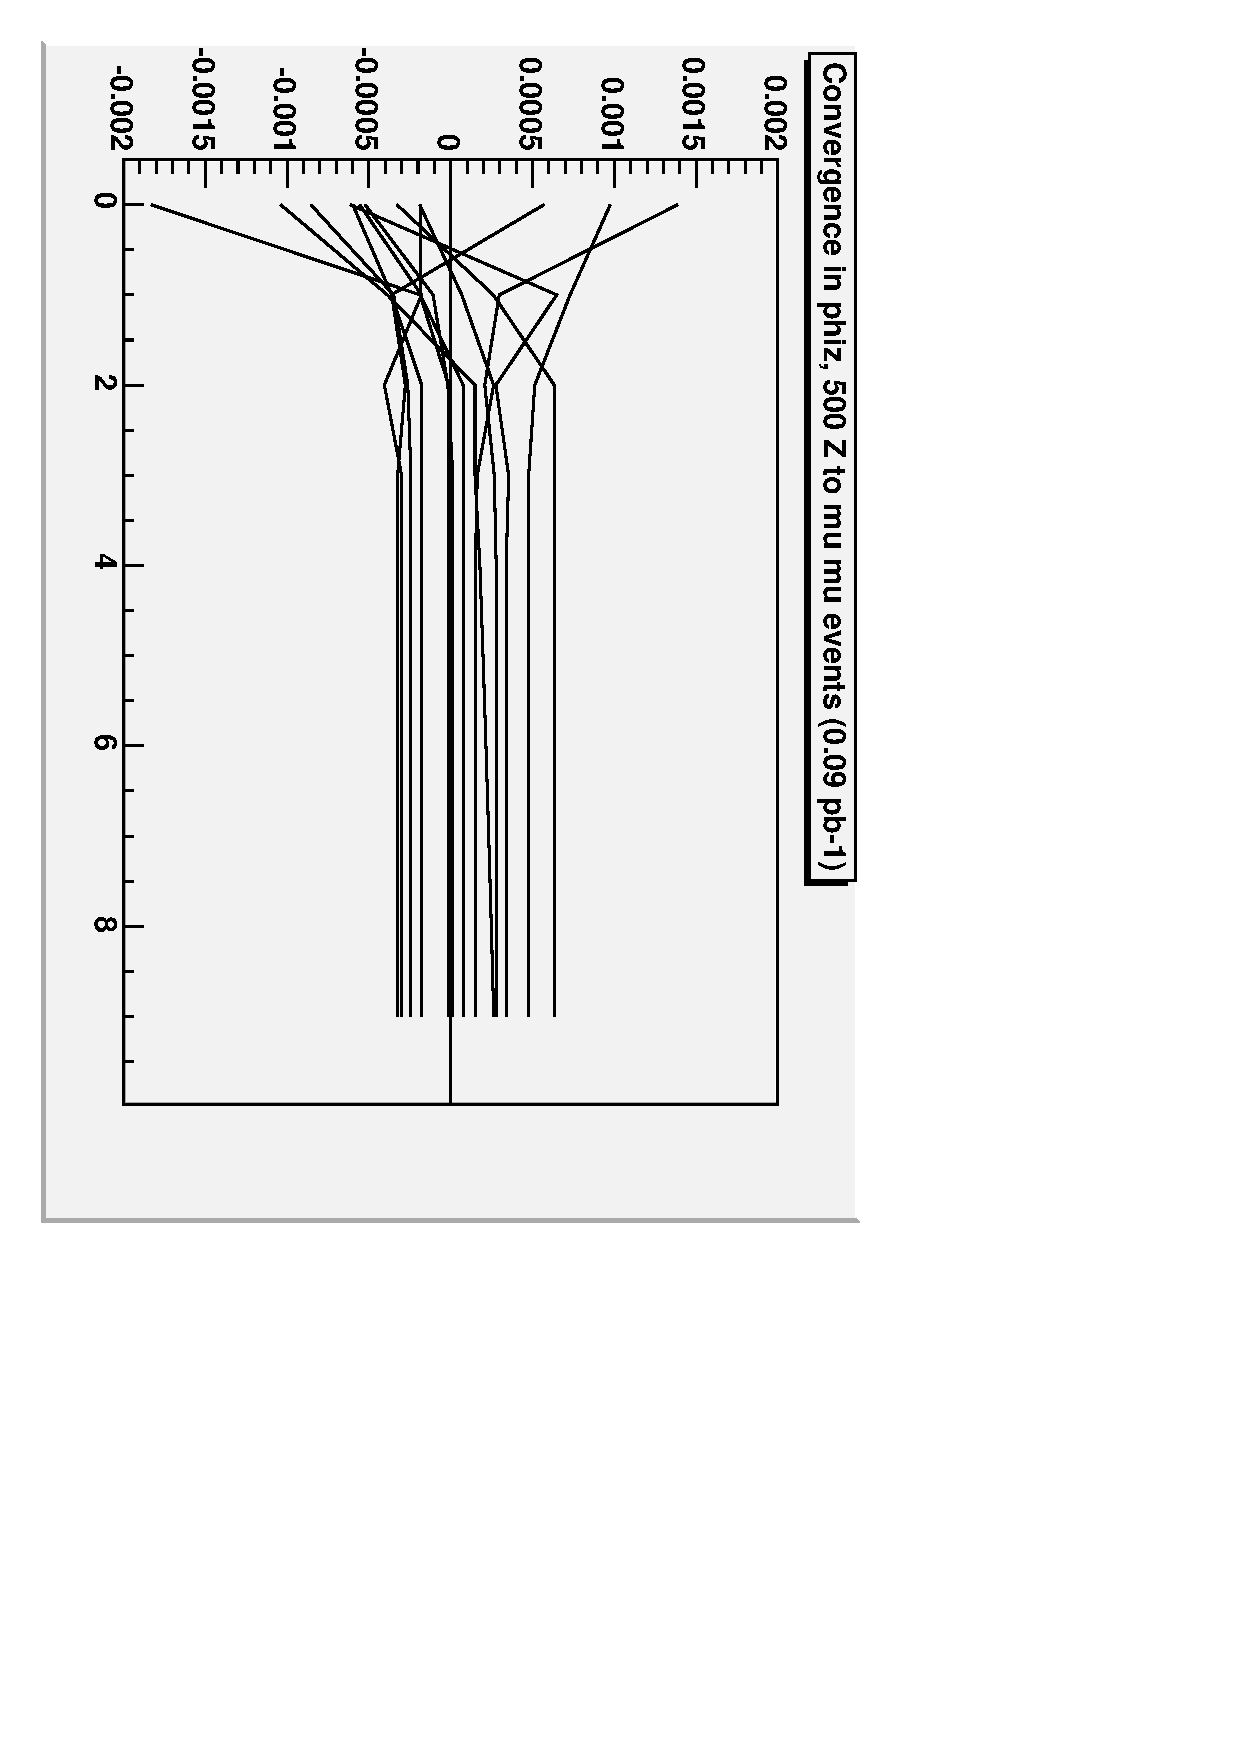
\includegraphics[height=\linewidth, angle=90]{phiz_conv_500.pdf} &
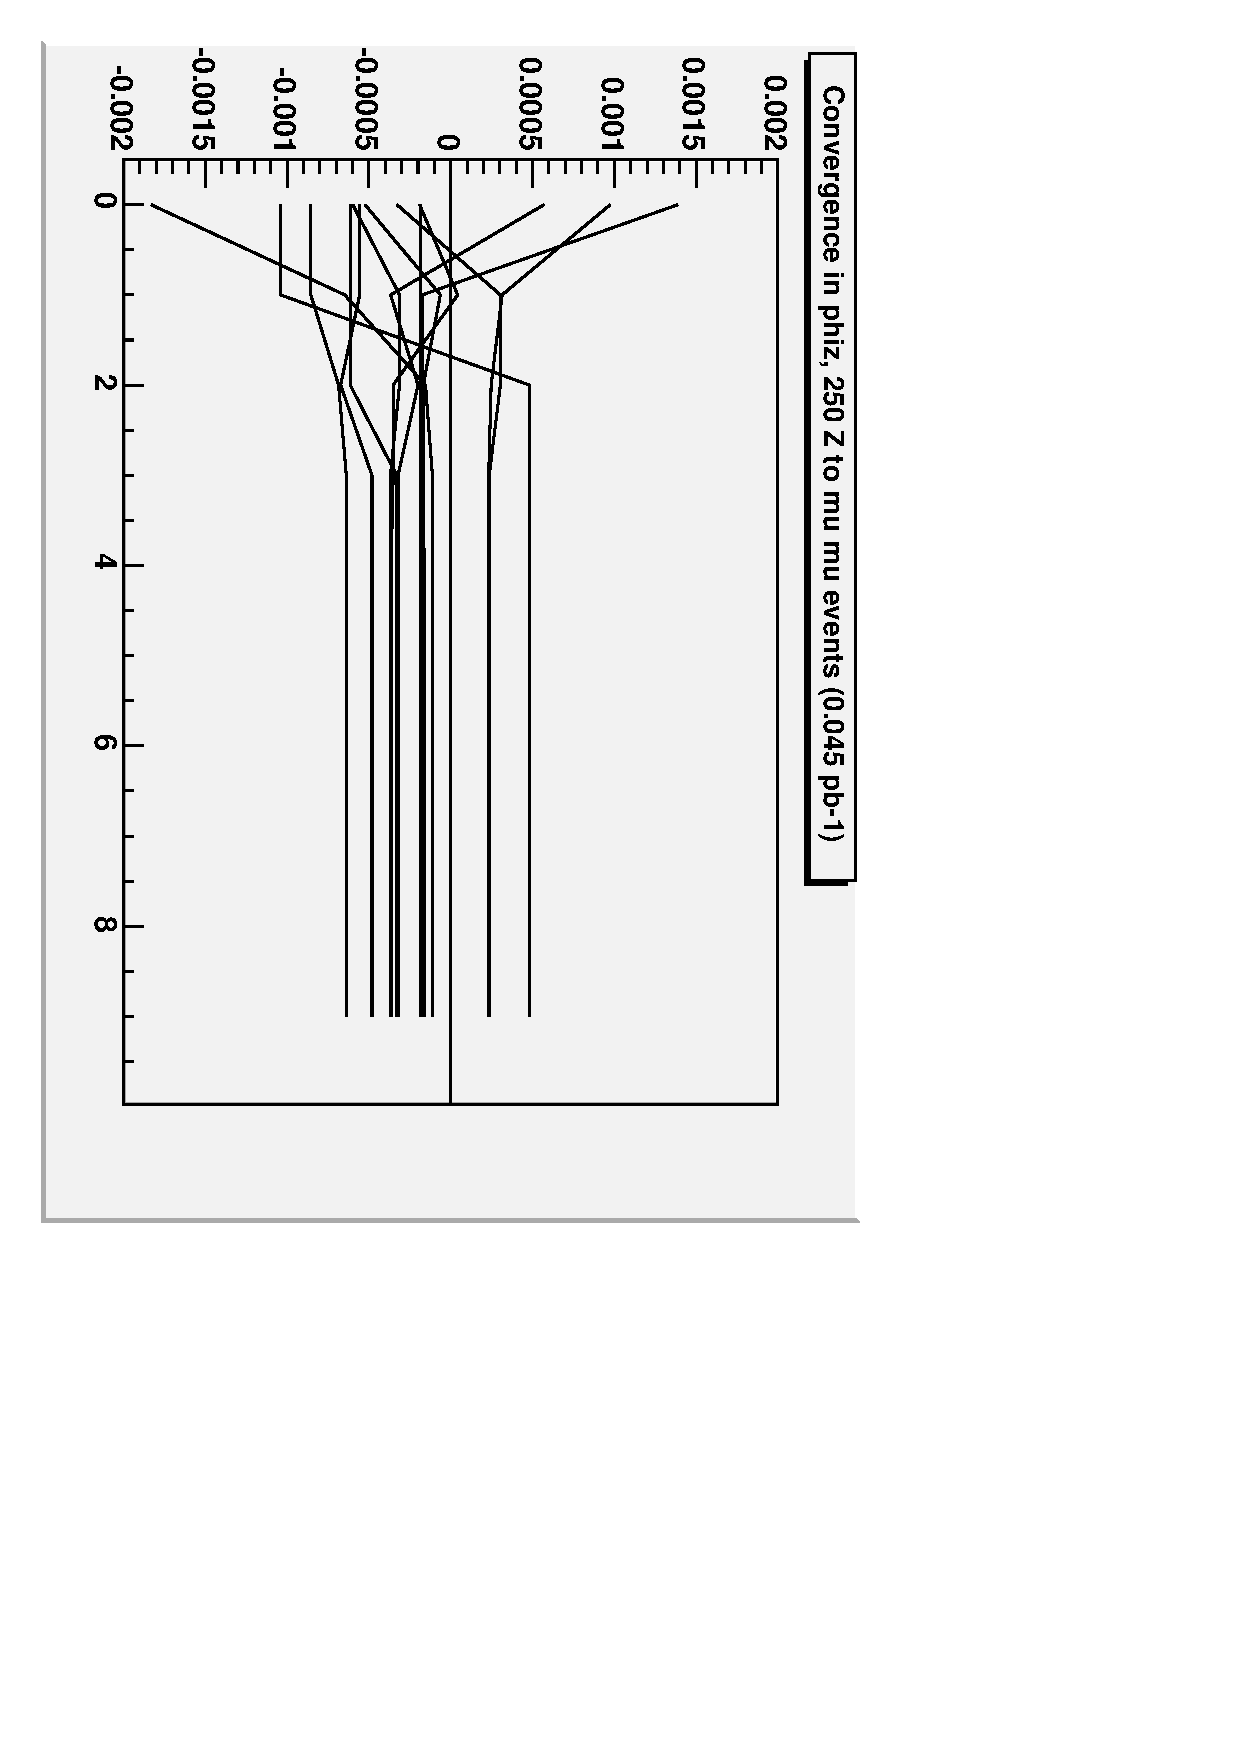
\includegraphics[height=\linewidth, angle=90]{phiz_conv_250.pdf}
\end{tabular}
\end{center}
\end{frame}

\begin{frame}
\frametitle{Alignment quality vs data used}
\begin{itemize}
\item RMS (not stdev!) of 13 disk/wheels times 10 trials, randomizing
muon alignment with each trial
\item Events used in each \#events bin are independent.
\end{itemize}

\vfill
\begin{center}
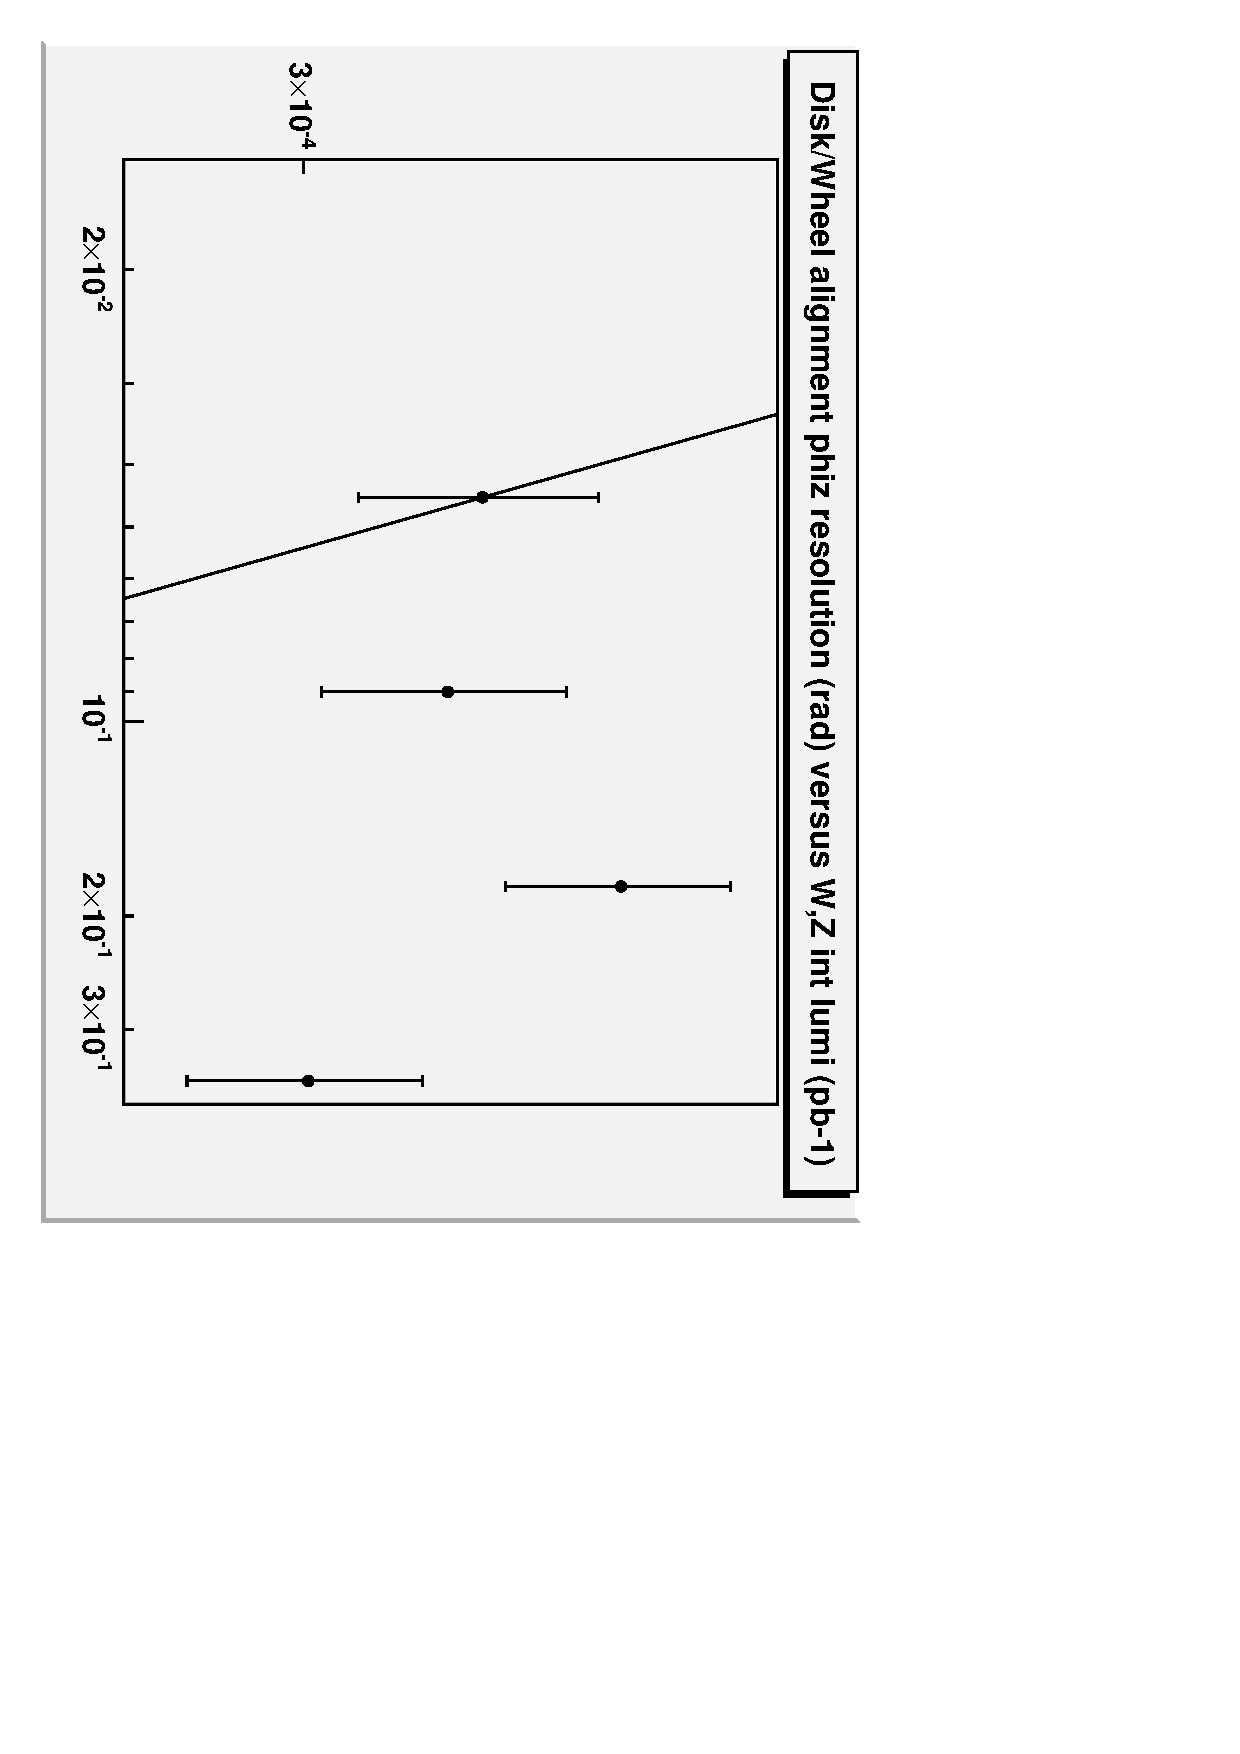
\includegraphics[height=0.6\linewidth, angle=90]{vsevents.pdf}
\end{center}

\vfill Early brick wall comes from internal misalignments.
\end{frame}

\begin{frame}
\frametitle{Conclusions}
\begin{itemize}\setlength{\itemsep}{0.5 cm}
\item Corrected all bugs, ready to move on to chamber-by-chamber alignments
\item Disk/wheel alignments are relatively insensitive to tracker misalignment (up to a few times expected short-term level); we can rely on globalMuon method
\item Chamber-by-chamber alignments ought to be more sensitive, but how much?  If not much, we may consider aligning the muon system to the tracker at an early stage
\item We need to be careful of RPC hits: they can bias alignments toward ideal
\end{itemize}
\label{numpages}
\end{frame}

\end{document}
